\begin{surferPage}[六次曲線(30 尖點)]{巴斯帶30尖點的六次曲線}
在沃爾夫·巴斯(Wolf Barth)構造了具有最多奇異點($65$個)的六次曲面之後,他的兩個學生也構造了創世界紀錄的更高次數的曲面。巴斯開始考慮對給定的次數的曲面可以構造最多個尖點的問題。
他的具有65個 $A_1^{+-}$型(雙錐型)奇異點的六次曲面可以用來構造尖點。這便產生了30個\[P_6 - \alpha \cdot K^3=0.\]其中$P_6$是正二十面體中與構造巴斯六次曲面時相同的一個對稱面,$K$同樣是單位球面。

    \vspace*{-0.4em}
    \begin{center}
      \begin{tabular}{c@{\ }c@{\ }c@{\ }c}
        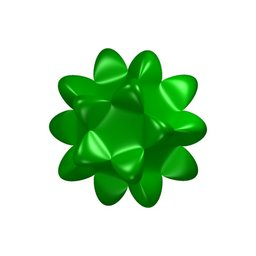
\includegraphics[height=1.2cm]{./../../common/images/barthsextic_30A2}
        &
        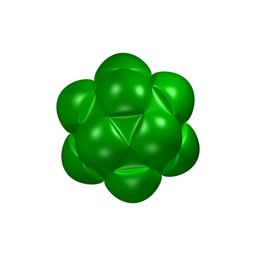
\includegraphics[height=1.2cm]{./../../common/images/barthsextic_30A2_3}
        &
        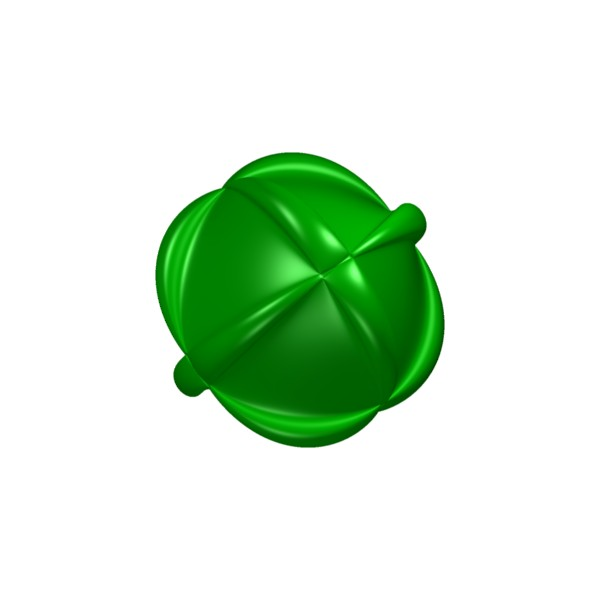
\includegraphics[height=1.2cm]{./../../common/images/barthsextic_30A2_5}
        &
        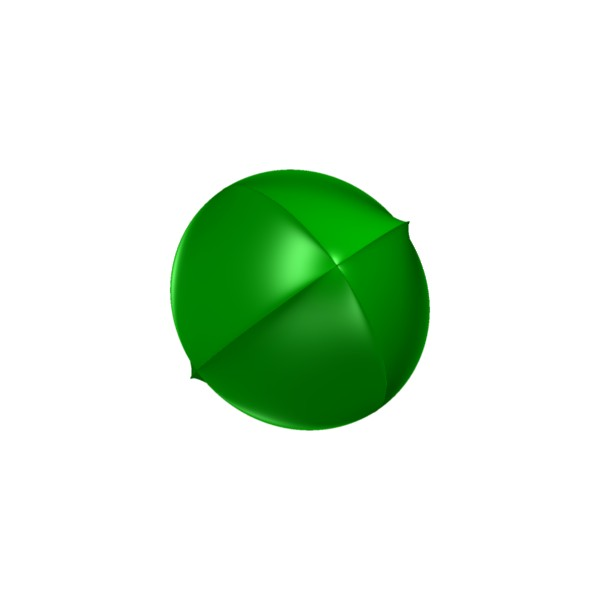
\includegraphics[height=1.2cm]{./../../common/images/barthsextic_30A2_6}
      \end{tabular}
    \end{center}
    \vspace*{-0.3em}

這是六次曲面上實尖點數當今世界紀錄最多的一個例子,它的複尖點個數是$36$。
\end{surferPage}
